%%%%%%%%%%%%%%%%%%%%%%%%%%%%%%%%%%%%%%%%%%%%%%%%%%%%%%%%%%%%%%%%%%%%%%
%     File: ExtendedAbstract_resul.tex                               %
%     Tex Master: ExtendedAbstract.tex                               %
%%%%%%%%%%%%%%%%%%%%%%%%%%%%%%%%%%%%%%%%%%%%%%%%%%%%%%%%%%%%%%%%%%%%%%

\section{Experiments}
\label{sec:experiments}

This section presents our comprehensive experimental evaluation of Aerial-D through both model training and cross-dataset generalization studies. We begin by describing our model architecture and training configuration, then present extensive evaluation results demonstrating the effectiveness of models trained on our dataset when applied to existing aerial referring segmentation benchmarks. Our experiments include ablation studies that examine the individual contributions of different expression enhancement strategies, providing insights into the optimal training configurations for various target domains.

\subsection{Model Architecture}
\label{subsec:model_architecture}

Our approach implements the RSRefSeg architecture\cite{chen2025rsrefseg}, which combines text and visual understanding for precise object segmentation in aerial imagery. The architecture leverages two robust vision foundation models: SigLIP2\cite{siglip2} for vision-language encoding and SAM\cite{sam} for mask generation. We implemented this architecture from scratch in PyTorch, employing LoRA (Low-Rank Adaptation)\cite{lora} for efficient fine-tuning while maintaining strong pre-trained representations from the foundation models. The model targets query and value projection layers in both vision encoders and query, key, value, and output projection layers in the text encoder.

\subsection{Experimental Setup}
\label{subsec:experimental_setup}

Our training configuration uses a batch size of 4 with gradient accumulation steps of 2, achieving an effective batch size of 8 samples. The model employs the SigLIP2-SO400M model for vision-language encoding and SAM-ViT-Base for mask generation. Training uses AdamW optimizer\cite{adamw} with initial learning rate of 1e-4, weight decay of 0.01, and polynomial learning rate decay with power factor 0.9. Mixed-precision computation and gradient clipping with maximum norm of 1.0 ensure training stability. All images are resized to 384×384 pixels to match SigLIP2 input requirements. Historic filters are applied on-the-fly during training to randomly present grayscale, grain/contrast roll-off, or sepia/noise variants without fixed per-image probabilities.

Our experimental design centers on training models using Aerial-D and evaluating performance through cross-dataset evaluation on three established aerial referring segmentation benchmarks: RefSegRS, RRSIS-D, and NWPU-Refer. This cross-evaluation approach validates the generalization capabilities of models trained on our dataset when applied to different aerial imagery domains.

\subsection{Evaluation Results}
\label{subsec:evaluation_results}

Our evaluation demonstrates the effectiveness of training a unified model on multiple datasets. The combined training performance evaluation in Table \ref{tab:combined_training_results} shows our main experimental results, where the model is trained on all five datasets (Aerial-D, RRSIS-D\cite{liu2024rotated}, NWPU-Refer\cite{yang2024large}, RefSegRS\cite{yuan2023rrsis}, and Urban1960SatSeg\cite{hao2025urban1960satseg}) and evaluated across different domains. This approach enables the model to leverage the diversity of expression styles and object categories across datasets while maintaining strong performance on each evaluation set.

% Combined training performance table
\begin{table*}[t]
\centering
\caption{Combined Training Performance Evaluation - Model Trained on All Dataset Train Sets (Historic-filtered results in \textcolor{blue}{blue})}
\label{tab:combined_training_results}
\begin{tabular}{@{}lcccccccc@{}}
\toprule
\textbf{Dataset} & \textbf{IoU@0.5} & \textbf{IoU@0.7} & \textbf{IoU@0.9} & \multicolumn{2}{c}{\textbf{mIoU}} & \multicolumn{2}{c}{\textbf{oIoU}} \\
\cmidrule(lr){5-6} \cmidrule(lr){7-8}
 & & & & \textbf{Orig.} & \textbf{Hist.} & \textbf{Orig.} & \textbf{Hist.} \\
\midrule
Aerial-D & -- & -- & -- & -- & \textcolor{blue}{--} & -- & \textcolor{blue}{--} \\
RRSIS-D & 68.51\% & 53.16\% & 18.74\% & 60.01\% & \textcolor{blue}{55.20\%} & 71.48\% & \textcolor{blue}{68.26\%} \\
NWPU-Refer & 38.64\% & 25.68\% & 6.64\% & 35.81\% & \textcolor{blue}{30.17\%} & 51.77\% & \textcolor{blue}{48.31\%} \\
RefSegRS & 36.43\% & 9.74\% & 1.39\% & 36.75\% & \textcolor{blue}{24.53\%} & 44.41\% & \textcolor{blue}{30.21\%} \\
Urban1960SatSeg & 74.80\% & 58.74\% & 28.46\% & 67.72\% & N/A & 86.43\% & N/A \\
\bottomrule
\end{tabular}
\end{table*}


\subsection{Aerial-D Generalization Results}
\label{subsec:ablation_studies}

To evaluate the individual contributions of different expression enhancement strategies, we conduct an ablation study comparing models trained on different subsets of Aerial-D. The primary motivation is to determine whether the LLM enhancement process positively impacts model performance and to quantify the benefits of each enhancement type. Our training set contains approximately 371K rule-based expressions, 364K language variation expressions, and 382K unique visual detail expressions, totaling 1.12M training expressions.

To ensure fair comparison across training configurations, we carefully control the total number of training samples each model observes. The individual subset models train for multiple epochs to match the sample count of the combined dataset trained for fewer epochs, preventing performance differences from arising simply from training data quantity rather than quality and diversity.

% Ablation expression types table with explicit epochs and samples
\begin{table*}[t]
\centering
\caption{Aerial-D Generalization Results Across Four Datasets}
\label{tab:ablation_expression_types}
\resizebox{\textwidth}{!}{%
\begin{tabular}{@{}lcc|cc|cc|cc|cc@{}}
\toprule
\multirow{2}{*}{\textbf{Training Configuration}} & \multirow{2}{*}{\textbf{Samples}} & \multirow{2}{*}{\textbf{Epochs}} & \multicolumn{2}{c|}{\textbf{Aerial-D}} & \multicolumn{2}{c|}{\textbf{RefSegRS}} & \multicolumn{2}{c|}{\textbf{RRSIS-D}} & \multicolumn{2}{c}{\textbf{NWPU-Refer}} \\
\cmidrule(lr){4-5} \cmidrule(lr){6-7} \cmidrule(lr){8-9} \cmidrule(lr){10-11}
 & & & % \textbf{Pass@0.7} & 
\textbf{mIoU} & \textbf{oIoU} & % \textbf{Pass@0.7} & 
\textbf{mIoU} & \textbf{oIoU} & % \textbf{Pass@0.7} & 
\textbf{mIoU} & \textbf{oIoU} & % \textbf{Pass@0.7} & 
\textbf{mIoU} & \textbf{oIoU} \\
\midrule
Rule-based Only & 371K & 4 & % 26.81\% & 
34.57\% & 39.31\% & % 2.55\% & 
3.73\% & 0.55\% & % 29.89\% & 
34.22\% & 36.46\% & % 13.62\% & 
16.78\% & 13.70\% \\
Enhanced Only & 364K & 4 & % 36.39\% & 
46.45\% & 56.99\% & % \textbf{3.02\%} & 
5.75\% & 4.99\% & % \textbf{35.63\%} & 
\textbf{41.63\%} & \textbf{42.48\%} & % \textbf{16.90\%} & 
21.89\% & 16.68\% \\
Unique Expressions Only & 382K & 4 & % 35.75\% & 
46.54\% & 63.02\% & % 2.55\% & 
18.32\% & 8.37\% & % 20.86\% & 
31.78\% & 33.73\% & % 15.91\% & 
\textbf{24.68\%} & \textbf{29.22\%} \\
Combined All & 1,118K & 2 & % \textbf{39.54\%} & 
\textbf{49.33\%} & \textbf{64.30\%} & % 1.86\% & 
\textbf{18.80\%} & \textbf{8.58\%} & % 23.39\% & 
34.07\% & 34.80\% & % 15.91\% & 
24.57\% & 28.27\% \\
\bottomrule
\end{tabular}%
}
\end{table*}

The results demonstrate that the combined model, utilizing all expression types, achieves the best performance across evaluation metrics on Aerial-D. Notably, different subsets show varying benefits for different target datasets: Enhanced Only performs best on RRSIS-D, while Unique Expressions Only excels on NWPU-Refer. This indicates that smaller, focused subsets can be more data-efficient and faster to train than the full combined dataset, while still achieving competitive or superior performance on specific target domains.


\subsection{Distillation Ablation: Gemma3 vs. o3 Model Comparison}
\label{subsec:distillation_ablation}

We evaluate the effectiveness of our knowledge distillation approach by comparing Gemma3\cite{gemma3}-enhanced expressions with those generated directly by the o3 model\cite{o3}. This comparison demonstrates both the quality improvements achieved through distillation and the significant cost advantages of using the distilled model for large-scale annotation generation.

To validate the effectiveness of our knowledge distillation approach, we conduct a qualitative comparison between our fine-tuned Gemma3 model (distilled from o3 using 500 samples) and the vanilla Gemma3 model without any exposure to aerial imagery or referring segmentation tasks. This ablation study demonstrates the significant impact of domain-specific fine-tuning on reducing hallucinations and improving the quality of generated referring expressions.

The comparison reveals stark differences in the models' ability to generate accurate, visually grounded expressions for aerial imagery. The vanilla Gemma3 model exhibits significant hallucination issues, often generating expressions that reference objects not present in the image, such as "airplane hangars" and "control towers" in residential areas. In contrast, the distilled Gemma3 model, trained on o3-generated expressions, produces accurate and grounded descriptions that correctly identify visible objects and their spatial relationships.

Figure \ref{fig:distillation_comparison} presents representative examples of this comparison across various aerial scenes and object categories. The results clearly illustrate how the fine-tuned model learned to avoid common hallucination patterns while maintaining the linguistic diversity and natural language quality that make the expressions useful for training robust segmentation models.

% Cost comparison table
\begin{table}[t]
\centering
\caption{Cost Analysis: Gemma3 vs. o3 Model for Large-Scale Annotation\protect\footnotemark}
\label{tab:cost_comparison}
\resizebox{\columnwidth}{!}{%
\begin{tabular}{@{}lcc@{}}
\toprule
\textbf{Model} & \textbf{Cost per request} & \textbf{Cost for 300K requests} \\
\midrule
o3 Model & \$0.020728 & \$6,218.32 \\
Distilled Gemma3 & \$0.000087 & \$26.01 \\
\midrule
\textbf{Savings} & \textbf{238× cheaper} & \textbf{\$6,192.31 (99.6\%)} \\
\bottomrule
\end{tabular}%
}
\end{table}
\footnotetext{Cost calculations based on API pricing — o3: \$2.00 per million input tokens, \$8.00 per million output tokens (OpenAI API platform); Gemma3-12B: \$0.035 per million input tokens, \$0.141 per million output tokens (OpenRouter inference provider). Average tokens per request: o3 (1,670.8 input, 2,173.3 output), Gemma3 (1,330.0 input, 284.7 output). Calculations based on 15 sample requests.}

The cost analysis demonstrates that using the distilled Gemma3 model provides substantial economic advantages for large-scale dataset generation. The upfront investment in distillation training pays off significantly when generating millions of annotations, making the approach both technically sound and economically viable for scaling to larger datasets.

\begin{figure*}[t]
\centering
\begin{minipage}{0.5\textwidth}
\centering
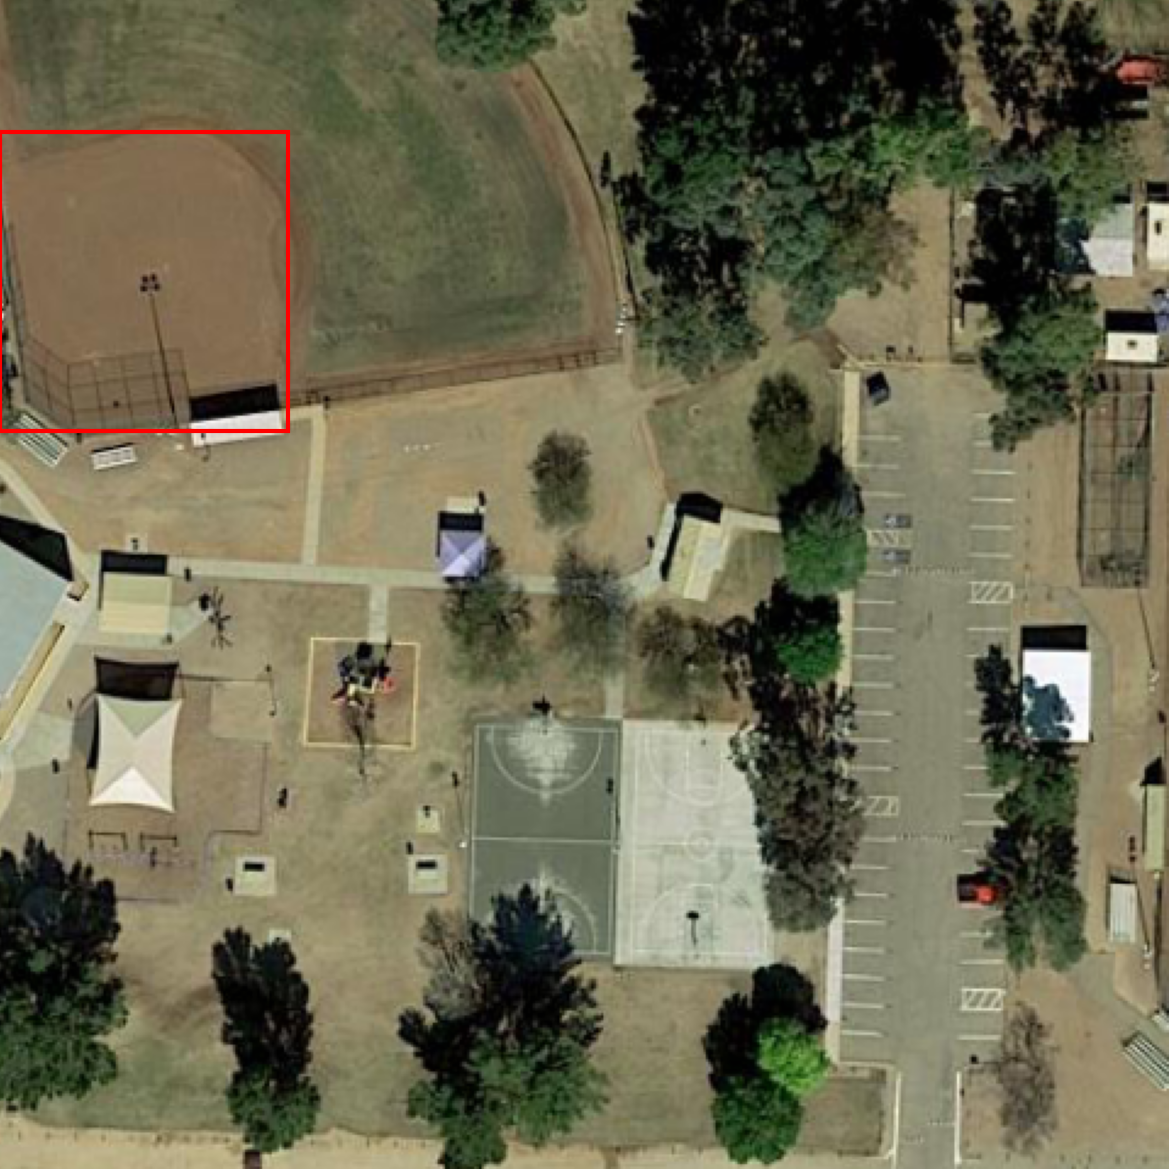
\includegraphics[width=0.65\textwidth]{./images/3llm.png}
\end{minipage}%
\begin{minipage}{0.5\textwidth}
\centering
\hspace{-1cm}
\raisebox{-0.3\height}{%
\footnotesize
\begin{tabular}{@{}p{2cm}p{5cm}@{}}
\toprule
\textbf{Expression Type} & \textbf{Example} \\
\midrule
Original & the orange baseball diamond in the top left \\
\midrule
o3 Enhanced & the orange baseball diamond with the light pole near home plate in the upper left \\
\midrule
Gemma3 Base & the bright orange baseball diamond to the left of another similar baseball diamond in the top left \\
\midrule
Gemma3-Aerial-12B & the orange baseball field with a chainlink fence surrounded by grass to the north and trees to the west \\
\bottomrule
\end{tabular}%
}
\end{minipage}
\caption{Qualitative comparison between o3, vanilla Gemma3 base model, and our fine-tuned Gemma3-Aerial-12B model on aerial imagery. The table shows how each model enhances the original rule-based expression, demonstrating the progression from basic rule-based descriptions through various levels of language model enhancement.}
\label{fig:distillation_comparison}
\end{figure*}


\subsection{Historic Filter Ablation Study}
\label{subsec:historic_ablation}

To isolate the impact of historic image filter training, we conduct an ablation study comparing models trained with and without historic filters applied during training. This study uses a model trained on all datasets (Aerial-D, RRSIS-D, NWPU-Refer, RefSegRS, and UrbanSatSeg1960) but without any historic image filters applied to the first four datasets - only UrbanSatSeg1960 contains historic imagery. The results in Table \ref{tab:historic_ablation_results} demonstrate the effectiveness of historic filter augmentation for improving model robustness to degraded image conditions commonly found in historical aerial photography.

% Historic filter ablation table
\begin{table*}[t]
\centering
\caption{Historic Filter Ablation Study - Model Trained on All Datasets Without Historic Filters (except UrbanSatSeg1960)}
\label{tab:historic_ablation_results}
\begin{tabular}{@{}lcccccccc@{}}
\toprule
\textbf{Dataset} & \textbf{IoU@0.5} & \textbf{IoU@0.7} & \textbf{IoU@0.9} & \multicolumn{2}{c}{\textbf{mIoU}} & \multicolumn{2}{c}{\textbf{oIoU}} \\
\cmidrule(lr){5-6} \cmidrule(lr){7-8}
 & & & & \textbf{Orig.} & \textbf{Hist.} & \textbf{Orig.} & \textbf{Hist.} \\
\midrule
Aerial-D & -- & -- & -- & -- & \textcolor{blue}{--} & -- & \textcolor{blue}{--} \\
RRSIS-D & -- & -- & -- & -- & \textcolor{blue}{--} & -- & \textcolor{blue}{--} \\
NWPU-Refer & -- & -- & -- & -- & \textcolor{blue}{--} & -- & \textcolor{blue}{--} \\
RefSegRS & -- & -- & -- & -- & \textcolor{blue}{--} & -- & \textcolor{blue}{--} \\
Urban1960SatSeg & -- & -- & -- & -- & N/A & -- & N/A \\
\bottomrule
\end{tabular}
\end{table*}
